\section{Results}

The results are split in two parts.
The first part is the context switching time value measured by our benchmarking framework.
For the second part, we have measured again the real context switching time with the oscilloscope the same way as for the reference measurement.

\paragraph{Context switching time measured by our framework} 
The value measured by our framework is represented in the table \ref{tab:framework-measurement}.

\begin{table}[!h]
  \centering
  \begin{tabular}{llll}
                        & \multicolumn{3}{c}{Time ($\mu$s)}          \\ \cline{2-4} 
                        & \multicolumn{1}{c}{Mean} & Min  & Max  \\ \cline{2-4} 
  From task 1 to task 2 & 7812                     & 7812 & 7812 \\
  From task 2 to task 1 & 7812                     & 7812 & 7812
  \end{tabular}
  \caption{Context switching time measured by our benchmarking framework}
  \label{tab:framework-measurement}
  \end{table}

\paragraph{Context switching time measured by the oscilloscope}
Using the same setup as for the reference measurement, we have measured again the real context switching time.
The figure \ref{fig:framework-value-wave} shows the voltage measured by the oscilloscope while using our framework.
The table \ref{tab:framework-measurement} shows the duration of the two context switchings and the two tasks.

\begin{figure}[!ht]
  \centering
  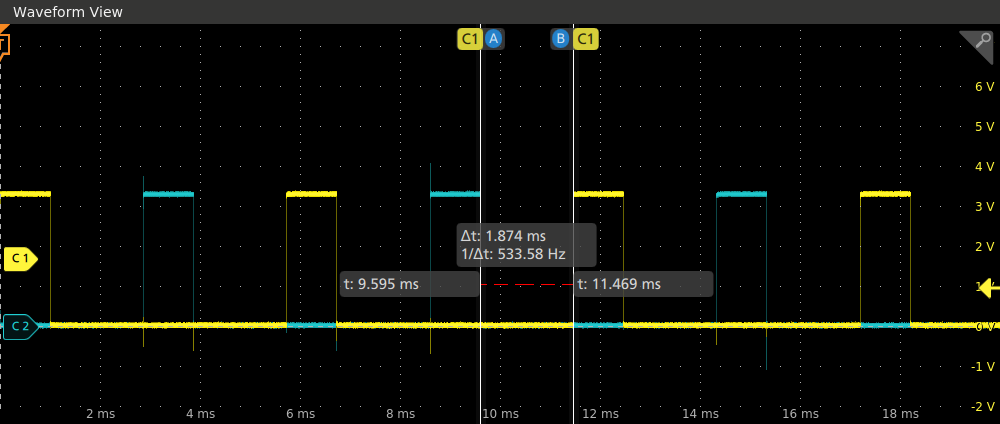
\includegraphics[scale=0.5]{assets/framework-value-wave.png}
  \caption{\label{fig:framework-value-wave}Voltage measurement of the two GPIOs; Each color represents a task}
\end{figure}

\begin{table}[!ht]
  \centering
  \begin{tabular}{llll}
                        & \multicolumn{3}{c}{Time ($\mu$s)}                             \\ \cline{2-4} 
                        & \multicolumn{1}{c}{Mean} & Min  & \multicolumn{1}{c}{Max} \\ \cline{2-4} 
  From task 1 to task 2 & 1864                     & 1863 & 1866                    \\
  From task 2 to task 1 & 1865                     & 1862 & 1866                    \\
  Duration of task 1    & 1003                     & 1003 & 1003                    \\
  Duration of task 2    & 1003                     & 1003 & 1003                   
  \end{tabular}
  \caption{Context switching times and task durations measured with the oscilloscope Tektronix MSO 56 using our framework}
  \label{tab:framework-measurement}
\end{table}

\subsection{Discussion}

By comparing with our reference measurement, the first assessment we can make is that our benchmarking framework does not compute the context switching time correctly.
The framework measure a context switching time of 7812 $\mu$s where we expect a value of 14.68 $\mu$s.

Second assessment we can make is that our framework add a huge overhead.
When comparing the figure \ref{fig:measurement-value-wave} with the figure \ref{fig:framework-value-wave}, the overhead is largely visible.
By comparing the values measured by the oscilloscope, the reference measurement and the real context switching time while using our framework, we see that our framework add an overhead of 1850 $\mu$s.
The table \ref{tab:measurements-comparison} shows this comparison.

\begin{table}[!ht]
  \centering
  \begin{tabular}{lll}
                        & \multicolumn{2}{c}{Time ($\mu$s)}                                     \\ \cline{2-3} 
                        & \multicolumn{1}{c}{No framework} & Framework \\ \cline{2-3} 
  From task 1 to task 2 & 14.68                                     & 1864                  \\
  From task 2 to task 1 & 14.88                                     & 1865                  \\
  Duration of task 1    & 1003                                      & 1003                  \\
  Duration of task 2    & 1003                                      & 1003                 
  \end{tabular}
  \caption{Comparison of the oscilloscope measurements}
  \label{tab:measurements-comparison}
\end{table}

\paragraph{Limitations of the framework}

As the results show, our framework suffers from several limitations.

First, the devices can not compute the context switching time with enough precision.
This lack of precision is due of the speed of the device clock that is not high enough.
In our experiment, the Zolertia RE-MOTE used with Contiki could only use a timer with 128 ticks per second or 1 tick every 7812 $\mu$s.

Second, our framework output its computed value through serial port.
Printing out at least 32 characters for every context switch on the serial port even at 250 kbit/s took 1.2ms.
One optimization could be to reduce the number of bits send or use a cache.